\documentclass{scrartcl} 
%\documentclass[a4paper]{article}
%\usepackage{a4wide}

\usepackage[ngerman,english]{babel}
 \usepackage[T1]{fontenc}
\usepackage{lmodern}
\usepackage[applemac]{inputenc}

\usepackage{amsmath}
\usepackage{amssymb}
\usepackage{amstext}
\usepackage{amsthm}

\usepackage{fancyhdr}
\usepackage{paralist}

\usepackage{mathtools}


\usepackage{hyperref}


\usepackage{graphicx}


\usepackage{wrapfig}


% PSEUDOCODE

\usepackage[ruled]{algorithm2e}


% C++ CODE

\usepackage{listings}
\usepackage{xcolor}
\definecolor{lbcolor}{rgb}{0.9,0.9,0.9}

\lstdefinestyle{customc}{
  belowcaptionskip=1\baselineskip,
  breaklines=true,
  %frame=LR,
  %xleftmargin=\parindent,
  language=C,
  showstringspaces=false,
  basicstyle=\footnotesize\ttfamily,
  keywordstyle=\bfseries\color{green!40!black},
  commentstyle=\itshape\color{purple!40!black},
  identifierstyle=\color{blue},
  stringstyle=\color{orange},
}

\lstdefinestyle{customcpp}{
	backgroundcolor=\color{lbcolor},
    	tabsize=4,
    	language=[GNU]C++,
        basicstyle=\tiny,%{\scriptsize},
        upquote=true,
        %aboveskip={1.5\baselineskip},
        columns=fixed,
        showstringspaces=false,
        extendedchars=false,
        breaklines=true,
        prebreak = \raisebox{0ex}[0ex][0ex]{\ensuremath{\hookleftarrow}},
        frame=single,
        numbers=left,
        showtabs=false,
        showspaces=false,
        showstringspaces=false,
        identifierstyle=\ttfamily,
        keywordstyle=\color[rgb]{0,0,1},
        commentstyle=\color[rgb]{0.026,0.112,0.095},
        stringstyle=\color[rgb]{0.627,0.126,0.941},
        numberstyle=\color[rgb]{0.205, 0.142, 0.73},
}

\lstset{escapechar=@,style=customcpp}


% TIKZ DIAGRAMS

\usepackage{tikz}
\usetikzlibrary{arrows}
\usetikzlibrary{positioning}

\tikzset{
    block/.style={
           rectangle,
           rounded corners,
           draw=black, very thick,
           minimum height=2em,
           inner sep=2pt,
           text centered,
           },
     block2/.style={
           %rectangle,
           %rounded corners,
           fill=black!20,
           %draw=black, very thick,
           minimum height=2em,
           inner sep=2pt,
           text centered,
           },
     frameless/.style={
           %rectangle,
           %rounded corners,
           %draw=black, very thick,
           minimum height=2em,
           inner sep=2pt,
           text centered,
           },
}

\usepackage{tikz-cd}
\tikzset{
  shift left/.style ={commutative diagrams/shift left={#1}},
  shift right/.style={commutative diagrams/shift right={#1}}
}



\DeclareMathOperator*{\esssup}{ess.sup}
\DeclareMathOperator*{\defgl}{\vcentcolon=}


%\pagestyle{fancy}
%\fancyhead[L]{Seminar \glqq Optimale Steuerung\grqq\\ Prof. Brokate, Prof. Kuttler} %Kopfzeile links
%\fancyhead[C]{} %zentrierte Kopfzeile
%\fancyhead[R]{10. Dezember 2013\\ Manuel Demmeler} %Kopfzeile rechts
\title{\vspace{-1.3cm} \textmd{\normalsize{High Performance Computing Project}}\\ Parallelization of the Probabilistic Roadmap Method with GPU Acceleration}
\date{}
\author{Manuel Demmeler}

%\thispagestyle{fancy}

\newcommand{\3}{ ^{3\times3} }
\newcommand{\R}{\mathbb{R}}
\newcommand{\N}{\mathbb{N}}
\newcommand{\M}{\mathbb{M}}
\newcommand{\Sym}{\mathbb{S}^3}
\newcommand{\Mpos}{\M_+^3}
\newcommand{\Orth}{\mathbb{O}^3}
\newcommand{\norm}[1]{\left\lVert#1\right\rVert}
\newcommand{\abs}[1]{\left |#1\right |}
\newcommand{\ub}{\bar{u}}
\newcommand{\yb}{\bar{y}}
\newcommand{\scprod}[2]{\langle#1 , #2 \rangle}

%\vspace{-3.4cm}


\begin{document}
\maketitle

\section{Motivation}
In trajectory optimization with obstacles, it is often necessary to provide feasible initial trajectories. 
For example in robot motion planning, where the dimensions of the underlying spaces are rather high, this can be expensive. A further problem is that because of the transformation from work into configuration space, the obstacles are often no longer given in a closed form. An efficient approximative solution for this is using probabilistic roadmaps (PRMs).

In this project, a parallelized version of the PRM method has been developed in general.
The robotics application then was implemented as an special case of this with GPU support.


\section{Introduction}
\subsection{Problem Statement and the Sequential PRM Method}\label{algintro}
\newtheorem*{defi}{Definition}
\newtheorem*{alg1}{Algorithm}


The abstract problem treated here is to find a path in a d-dimensional space, which avoids intersecting obstacles. The area occupied by obstacles is given by an indicator function
\begin{equation*}
	I: \Omega \rightarrow \{0, 1\}
\end{equation*}
on a region \( \Omega = [ q_{min,1}, q_{max,1} ] \times ... \times  [ q_{min,d}, q_{max,d} ] \subset \R^d  \). Hence, the goal is to find a continuous curve
\begin{equation*}
	\Gamma: [0,1] \rightarrow \Omega
\end{equation*}
between a given start and endpoint, \(\Gamma(0)=q_b,\ \Gamma(1)=q_e \), 
such that
\begin{equation*}
	I(\Gamma(s))=0 \text{\ f.a.\ } s�\in [0,1].
\end{equation*}
The PRM algorithm now grows a graph \(G=(V,E)\) form points \(q_s\) and \(q_e\) by randomly sampling nodes \(v\in \Omega\) and inserting them into $V$.  Two nodes \(v,w \in V\) are connected by an edge, if they are near enough each other and the line between them is free from obstacles. The algorithm terminates, when there exists a path from \(q_s\) to \(q_e\) on G.
\begin{defi}
For two points \(q_1\) and \(q_2\) we define the connection with stepsize \(h>0\) as
	\begin{equation*}
		[q_1,q_2]_h \defgl \{ q = \lambda q_1+(1-\lambda) q_2\ |\ \lambda \in [0,1], \norm{q-q_1} \in \N_0 h \}.
	\end{equation*}
	We say, \(q_1\) and \(q_2\) are connected with stepsize \(h>0\), if
	\(I(q)=0\) for all \(q \in [q_1, q_2]_h\).
\end{defi}

\begin{algorithm} 
	\caption{Probabilistic Roadmap Algorithm}
	\KwData{ \(q_s, q_e\in \Omega, h>0, d_0>0\)}
	\KwResult{ \(q_s=q_1, ... ,q_n=q_e\in \Omega\), 
		such that all \(q_i\) and \(q_{i+1}\) are connected with stepsize \(h\)}
	Initialize graph \(G=(V,E)\) with \(V=\{q_s, q_e\}\) \\
	If \(q_s\) and \(q_e\) are connected, \(E \leftarrow\{ q_s, q_e\}\) \\
	\While{ there exists no path in G between \(q_s\) and \(q_e\)}{
		Sample \(q\in \Omega\) from a probability density  \(p(\ \cdot\ , G)\), resample until \(I(q)=0\) \\
		\For{ all nodes \(\tilde{q} \in V\), with \( \norm{q- \tilde q} \le d_0 \) }{
			\If { $q$ and $\tilde q$ connected with stepsize h} {
				\(E \leftarrow \{q, \tilde{q}\}\)
			}
		}
		\(V \leftarrow{q}\), if at least one edge was inserted \\
	}
	Determine the shortest path \(q_1, ... , q_n\in V\) on \(G\) from \(q_s\) to \(q_e\).
\end{algorithm}

The probability density \(p(\ \cdot\ ,G)\) (depending on the actual graph) can be for example first selecting randomly a node \(q_0 \in V\) and then sampling a new point \(q\) in the neighbourhood of \(q_0\). Theory about success probabilities and convergence results can be found in \cite{prmlec}, \cite{prm1} or \cite{prm2}.


\subsection{Application to Robotics}


\begin{figure}
    \centering
    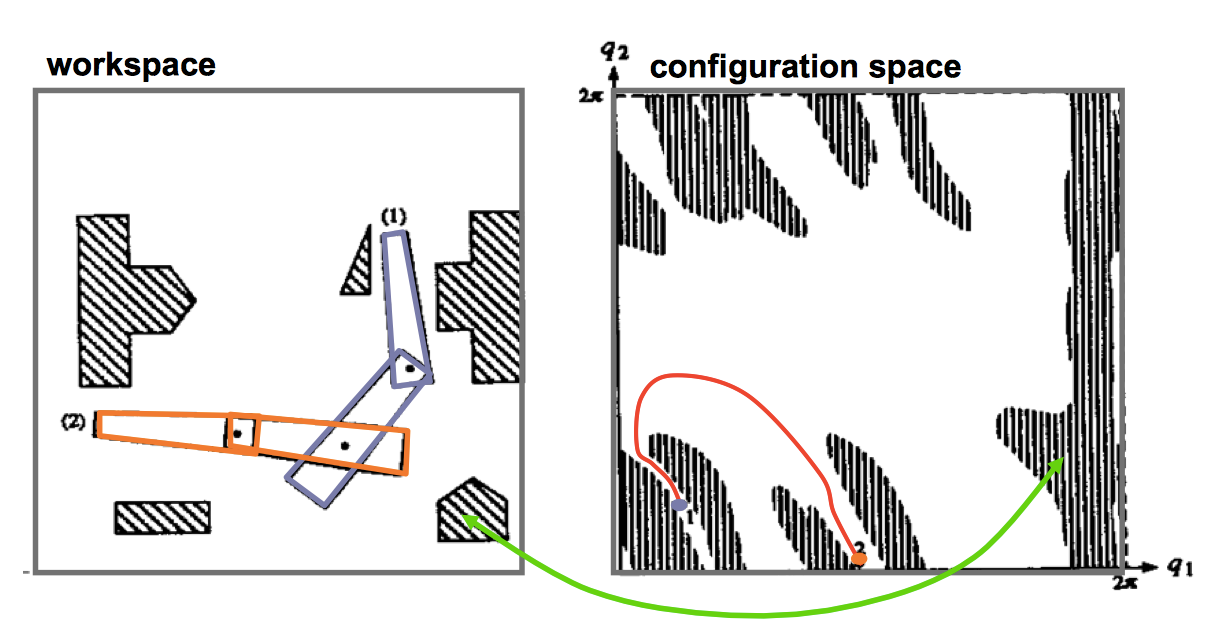
\includegraphics[width=0.8\textwidth]{configspacetrafo.png}
    \caption{Example from \cite{prmlec} for an indicator function in robotics. 
    		The real obstacles on the left are transformed 
		into occupied areas of the configuration space on the right.}
    \label{fig:awesome_image}
\end{figure}

In this project, the PRM algorithm is used to find trajectories for a robot arm, which avoid self collisions and collisions with obstacles in the environment.
Such trajectories can be expressed as functions describing the joint variables changing over time, that means as a curve in the configuration space with dimension equal to the number of degrees of freedom of the robot.
With this association, the trajectory finding problem becomes a path finding problem in the configuration space exactly of the form defined in the previous section.
The real obstacles transform into obstacles in the configuration space, given by the indicator function, that returns for a given vector of joint angles, if it is feasible or leads to a collision.


\newpage
\subsection{Project Overview}

Like in the stated robotics example, in many cases the most costly operation of the PRM algorithm are the many evaluations of the indicator function \(I(q)\), 
which however can be done independently for every new \(q\).
Therefore it is implemented in a vectorized way as a function \((q_1, ... , q_P) \mapsto (I(q_1),...,I(q_P))\) by a CUDA kernel, where every GPU thread computes one evaluation.
In the robotics case, this means, the direct kinematic and collision calculation are made on the GPU parallelly for different joint angle configurations.
Although this will the only major application in the project, the PRM solver and the configuration space are implemented separated from each other and connected by an interface to be free to simply add other applications. As an example and for testing, additionally a simple 2D configuration space is provided, 
whose indicator function is read from a black-and-white image.


\begin{center} 
\begin{tikzpicture}[auto]%node distance=0.5cm and 1.8cm]
	\node[block] (prm) {
		\begin{tabular}{c}
		\textbf{PRMSolver}\\
		generate nodes\\
		store graph
		\end{tabular}
	};
	\node [block, right=of prm] (config) {
		\begin{tabular}{c}
		\textbf{Configpace}\\
		indicator fct. \\
		interface
		\end{tabular}
	};
	\node [block, right=of config] (robo) {
		\begin{tabular}{c}
		\textbf{RobotConfigspace}\\
		robot kinematics\\
		collision detection
		\end{tabular}
	};
	\node [block, right=of robo] (gpu) {\textbf{GPU}};
	
	\path[-stealth,thick, shift left=1.0ex]	(prm) edge (config) ;
	\path[-stealth,thick, shift left=1.0ex]	(config) edge  (prm) ;
	\path[-stealth,thick, shift left=1.0ex]	(config) edge (robo);
	\path[-stealth,thick, shift left=1.0ex]	(robo) edge  (config);
	\path[-,thick]					(robo) edge (gpu);
\end{tikzpicture}
\end{center}


While the distribution of the indicator function to different CUDA threads is a first level of parallelization, 
a second level can be achieved by sampling and connecting several new nodes parallelly. 
This is more difficult, because all new nodes have to be connected 
and the graph data has to be updated on all processes. 
For this, different approaches have been implemented, which are described in chapter \ref{solver}.

Before that, chapter \ref{indicator} gives more details about the robotics indicator function.


%%%%%%%%%%%%%%%%%


\section{Implementation of an Indicator Function for Robot Arms}\label{indicator}

The probabilistic roadmap algorithm is applied  to create collision-free trajectories of a robot arm.
For a robot with given joint angles \(q_i\) one can calculate straightforwardly all positions and orientations  of the single parts of the robot.
For this, coordinate frames according to the Denavit-Hartenberg convention are used.
The coordinate frames of the single parts are described by transformation matrices 
$T_i \in R^{4x4}$, which transform points from the body frame into the world frame. They depend on the state $q=(q_1,...,q_d)$ of the robot and on the geometry of the joint angles given by the Denavit-Hartenberg parameters of the robot. 

The geometry of the robot parts is defined by a set of convex polytopes, each of them belonging to one of the robots coordinate frame. Applying the corresponding transformation $T_i$, its vertices can be transformed into the world frame. 
Environment obstacles are also defined by convex polytopes, given in the world frame.

Now the movement of the robot can be described by a curve $q(t) \in \R^d$ in the configuration space. It is collision-free, if at no time, any two polytopes of the robot intersect with each other or with the environment after being transformed into the world frame.
To apply the probabilistic roadmap algorithm, we express this by the indicator function

\begin{equation*}
	I(q)=
	\begin{cases}
		0,	& \text{ for no collision for all given pairs of polytopes } \\
		1,	& \text{ if at least one collision occurs }
	\end{cases}
\end{equation*}


The indicator function is implemented in a vectorized way as an CUDA kernel, which means that, given set of states $q^1,..,q^M$, the indicator function is evaluated for each state by one CUDA thread. Therefore, the kinematics and collision algorithm are implemented as device code for the use in the kernel.

It has to be noted that the trajectories \(q(t)\), the PRM algorithm will generate, are piecewise linear and therefore not differentiable. Hence, they have to be smoothed before the use on a robot. This is not part of the project. The task is only to generate feasible trajectories to be passed to an optimizer.

\subsection{Direct Kinematics}\label{dk}

The Denavit-Hartenberg (DH) convention is a method to describe the geometry of a robots joints, 
that is, how the transformations between the robots coordinate frames look like in dependency of its joint values $q_1,...,q_d$.
A robot consists of $d+1$ bodies each of which has a body fixed coordinate frame $B_i$, which is described by a transformation matrix $T_i$ into the world frame.
It is assumed that each joint is either rotational, that means an rotation around a fixed axis, 
or prismatic, a translation along an axis.
These joints may now be defined through DH parameters $a_{i-1}, \alpha_{i-1}, d_i, \theta_i \in \R$, $i=1,...,d$, 
by setting the relative transformations $T_{i-1,i}=T_{i-1}^{-1} T_{i}$ between two bodies to
\begin{equation}
	T_{i-1,i} = R_z(\theta_i) T_z(d_i) R_x(\alpha_{i-1}) R_x(a_{i-1})
\end{equation}
where $R_x, R_z$ are rotations and $T_x, T_z$ translations around the $x$ and $z$ axes.
With this and $T_0=I$, all transformations $T_i$ are determined.

The other way round, one can now show, that by an proper choice of the body frames, every robot with rotational or prismatic joints can be described by such a set of DH parameters, i.e. it exists a set of parameters, such that the above definition leads to the correct transformations for this robot.
For the exact calculations, see \cite{robodyn}.


\subsection{2D and 3D Geometry Library}

For the implementation of the kinematics and later the collision algorithm, a geometry library was written, based on the CUDA datatypes float2 for 2D vectors and float4 for 3D vectors.
To guarantee aligned access on the GPU, float4 is used instead of float3. Furthermore, as the geometric calculations made here are numerically not very critical, the usage of double precision has turned out to be not necessary.
The library contains hybrid host and device inline functions for common vector operations such as
\begin{lstlisting}
__host__ __device__ inline float4& operator += (float4& u, const float4& v);
__host__ __device__ inline float4& operator *=  (float4& u, const float f);
__host__ __device__ inline float4& add(const float4& u, const float4& v, float4& w);
\end{lstlisting}
Operators like $+$ or $*$ are not overloaded to prevent unnecessary temporary variables.

Transformation matrices are implemented as float4 arrays with inline functions for common matrix operations. Again operators with temporaries were avoided, wherever possible.
\begin{lstlisting}
class trafo4{
  public:
    float4 col[4];
    __host__ __device__ trafo4(){}
    __host__ __device__ trafo4(float a, float alpha, float q, float d);
    __host__ __device__ inline float4& apply(float4& u) const;
    __host__ __device__ inline float4& apply(const float4& u, float4& Tu) const;
    .
    .
    .
}
\end{lstlisting}

The second constructor implements the relative DH transformations.

\subsection{Polytopes}

To calculate the intersection between two convex polytopes, the here used Chung-Wang algorithm only needs their vertices 
and the data, which of them are connected by an edge. 
For this the adjacency matrix of the edge graph is stored compactly in compact row storage format.
\begin{lstlisting}
struct polytope4{
    float4* vertices;	//length n
    int n;
    //edges
    int* dsp;	//length n
    int* cnt;	//length n
    int* dest;	//length m
    int m;
};
\end{lstlisting}
It means, that for $i=0,...,n-1$ the vertices $dest[dsp[i]],...,dest[dsp[i]+cnt[i]-1]$ are the ones connected with vertex $i$ by an edge.
The polytopes used in this project are given by the user as convex hull of a list of vertices. However, to determine the edge graph only from the vertices is a nontrivial task, which is done by Matlab here using provided high level functions.


\subsection{Chung-Wang Collision Algorithm}

To check if two polytopes collide an algorithm by Chung and Wang is used here. It uses the separating vector theorem and tries to find a separating vector by iterative search. Furthermore, a sub-algorithm determines in each iteration from the candidate history, if it is still theoretically possible to find a separating vector. If not, it is returned a collision. If on the other side a separating vector is found, the algorithm can return no collision.
For detailed informations see \cite{chung} and \cite{ericson}, pp. 410-412.
The method is implemented as device code for the use on GPU kernels.
\begin{lstlisting}
__host__ __device__ int separating_vector_algorithm(const polytope4& P, const polytope4& Q, 
													const trafo4& tp, const trafo4& tq);
\end{lstlisting}
In our application, the polytopes are mostly parts of the robot, which are given in a body frame and have to be transformed into world frame according to section \ref{dk} first.
However, from the structure of the Chung-Wang algorithm drops out, that mostly only a small part of the polytopes vertices are needed for the computations. Therefore, it would be rather time wasting to transform all vertices before passing them to the algorithm. To avoid this, all polytopes are passed in their body frames together with their transformations and the algorithm transforms a vertex, whenever it occurs in calculations.
This is also the version proposed in \cite{chung}.




\subsection{Robot Kernel}

The robot configuration space is implemented in the form
\begin{lstlisting}
template<int ndof>
class RobotConfigspace : public Configspace<ndof>
{
public:
  RobotConfigspace(const Robot<ndof>* robot_,
                   const polytope *polys_,
                   const int* sys_,
                   const int N_,
                   const int *from_, const int *to_,
                   const int M_,
                   const float* mins_, const float* maxs_, const float dq_,
                   const int nbuf_);
  int init(const int ressource_rank=0, const int ressource_size=1);
  int indicator2(const float* qs, const float* qe, int *res, const int N, const int offset);
  .
  .
  .
private:
  const Robot<ndof>* robot; //host object
  Robot<ndof>* robotdev;    //GPU object
  collision4::polytope4data* polydata;    //host object
  collision4::polytope4data* polydatadev; //GPU object
  .
  .
  .
}
\end{lstlisting}
\begin{lstlisting}
__global__ void kernel_indicator2(const Robot<ndof>* robot,
                                  const collision4::polytope4data* polydata,
                                  const float* qs, int offsets,
                                  const float* qe, int offsete,
                                  int* res,
                                  const int* testpos, const int* testnum,
                                  int N, int numthreads);
\end{lstlisting}
where the constant geometry and robot data is loaded once at the beginning and copied to the GPU by an init function.
The indicator function gets as input a list of border points $q_{start}^j, q_{end}^j, j=0,...,N$ and checks now for each pair, if the indicator function is always 0 on the line in between.
\begin{equation}
	res[j]=\begin{cases}
		0	&\text{if $I(q)=0$ f.a. $q \in \left[qs[j], qe[j]\right]_{\Delta q}$} \\
		1	&else
	\end{cases}
\end{equation}
The border points are stored in structures of arrays.
\begin{equation}
\begin{aligned}
	q_{start}^j &= \left(qs[j],qs[j+\text{offset}],...,qs[j+(d-1)*\text{offset}]\right)^T\\
	q_{end}^j &= \left(qe[j],qe[j+\text{offset}],...,qe[j+(d-1)*\text{offset}]\right)^T
\end{aligned}
\end{equation}

As the PRMSolver only needs to know, which node points can be connected by a line, and not, which intermediate points are free in detail, this version delivers exactly the minimal necessary information. 
Furthermore, it saves CPU and communication time, because the intermediate points on the lines can be directly computed by the GPU threads and do not need to be exchanged.

Algorithms \ref{host} and \ref{kernel} show in pseudo code, how the work is split between host and device.


\begin{algorithm}\label{host}
	\KwData{qs, qe, N, offset}
	\KwResult{res}
	compute distances $d_j = \abs{q_{end}^j - q_{start}^j}$ \;
	testnum[j] = $d_j/{\Delta q}$: number of threads for each line \;
	testpos[j] = thread displacements \;
	reset res \;
	call kernel \;
	\caption{Host indicator function}
\end{algorithm}

\begin{algorithm}\label{kernel}
	\KwData{arrays qs, qe, testpos, testnum and threadindex}
	\KwResult{res}
	compute associated edge number $j$, defined by $testpos[j] \leq threadindex \le testpos[j]+testnum[j]$ \;
	$c = (threadindex - testpos[j]) / (testnum[k]-1) $ \;
	$q=c q_{start}^j + (1-c) q_{end}^j $ \;
	calculate robot kinematics $T_0(q), ..., T_d(q) $\;
	$res_{tmp} = 0; $ \;
	\For{all registered pairs pairs of polytopes $P, Q$}{
		$res_{tmp}=separating\_vector\_algorithm(P, T_{i_P}, Q, T_{i_Q})$ \;
		\If{$res_{tmp} \neq 0$}{
			$res[j]=res_{tmp}$ \;
			break \;
		}
	}
	\caption{Robot kernel: code for one thread}
\end{algorithm}

In order to overlap computation time of GPU and CPU, an asynchronous version of the indicator function was written. Here the function is divided into everything until the kernel launch and a function, which waits, until the kernel has finished and receives the result data.

\begin{lstlisting}
int indicator2_async(const float* qs, const float* qe, int *res, 
					 const int N, const int offset, int &request);
int indicator2_async_wait(int request);
\end{lstlisting}

The implementation also allows overlapping of multiple requests, for example two calls of the launch function and after this the two corresponding waiting calls. 
With this, it is possible to use the full computation time of the GPU.


\newpage
%%%%%%%%%%%%%%%%%%%%%%%%

\section{The PRM Solver}\label{solver}

The solver builds a first phase the roadmap graph from both the start and the end node, until it is connected.
It is always ensured that the graph consists of two connected components containing the start resp. the end node.
With this, it can be easily determined at each time, if the whole graph has become connected.

At the end, in a second phase, a shortest path from the start to the end node is searched by the Dijkstra algorithm.
It has shown, that this part needs a neglectable amount of time compared to building the graph.
Therefore, it is not parallelized here and the focus lies on the first phase.

\subsection{Storing the Graph}

Apart from the indicator function evaluation, the main problem in building the probabilistic roadmap is, that for each new node $q$ it have to be determined all possible neighbors. That is the set of all nodes $\tilde q$ of the graph, with $\norm{\tilde q - q} \le D$.
If no special order of the nodes is given, one has to calculate this norms for all nodes of the graph, which is rather time consuming.

Therefore, a special indexing is used here. 
The nodes are stored in a vector, which is organized in blocks with fixed sizes. The blocks are referred to by ids which are stored in a map.

\begin{lstlisting}
struct block{
	int pos;	 //! position of first vertex
	int num;	 //! current number of vertices stored
	block* next; //! if num==blocksize -> pointer to next block
};
\end{lstlisting}


\begin{lstlisting}
struct graph{
    std::map<int,block*> map; //map for accessing blocks
    std::vector<block> blocks;
    std::vector<float> qstorage; //length ndof*N
    int newblockpos;  //position of next new block
    int blocknum;     //number of used blocks
    .
    .
};
\end{lstlisting}

The key of an block is computed by the mapping
\begin{equation*}
	key(q) = \left\lfloor \frac{q_1}{H} \right\rfloor
\end{equation*}
such that $H>0$ becomes a parameter to adjust the grid density.
This has to be chosen so large that enough nodes are stored in one block in order to have efficient memory access.
On the other side, the smaller it is, the less unnecessary computations have to be done for the neighborhood requests.
For illustration of the structure, the following pseudocode shows the insertion of a node.

\begin{algorithm}[H]
	\KwData{$q\in\R^d$}
	Compute key=key(q)\\ 
	\eIf{key exists in map}{
		block=map[key]\\ 
		\While{ block full }{
			block=block->next
		}
	}{
		insert new block at map[key]
	}
	Insert node into block
	\caption{Inserting a node}
\end{algorithm}

For getting the neighbors of a node $q$ it is then enough to look at the keys from $key(q-cD)$ to $key(q+cD)$. For $D=H$, $c=1$ is possible.
The key mapping could be generalized by taking more components of $q$ into account, but that was not done here.

\subsection{Parallelization Models}

The parallelization is done with MPI. All processes store their own versions of the graph, which are hold up to date between each other.
Furthermore, it is assumed that every process has its own GPU.
The work of the single MPI processes could be parallelized further with OpenMP, but this has not been done here.
Instead, different approaches to distribute the work over several GPUs have been investigated.

\subsubsection*{Version 1} 

In the first approach, that has been evaluated, every process generates new nodes independently from each other.
Then the possible neighbors are determined and the connections, which have to be tested.
The indicator function is called and returns the edge data.
After this, the graph must be synchronized between all processes, which needs an all-to-all communication.
As the graph building phase does not need the edge data, it is sufficient to exchange only the nodes and collect the edges at the end.

	
	\begin{center}
\begin{tikzpicture}[auto, node distance=0.5cm and 1.8cm]
	\node[block, minimum width=3cm] (prm) {
		\begin{tabular}{c}
		\textbf{PRMSolver 1}
		\end{tabular}
	};
	
	\node[frameless, below=of prm, minimum width=3cm] (space) {$\vdots$};
	
	\node[block, below=of space, minimum width=3cm] (prm2) {
		\begin{tabular}{c}
		\textbf{PRMSolver n}
		\end{tabular}
	};
	
	\node [block, right=of prm] (config) {
		\begin{tabular}{c}
		\textbf{Configpace 1}
		\end{tabular}
	};
	\node[frameless, below=of config] (space2) {$\vdots$};
	\node [block, below=of space2] (config2) {
		\begin{tabular}{c}
		\textbf{Configpace n}
		\end{tabular}
	};
	
	
	
	\node [block, right=of config] (gpu) {\textbf{GPU 1}};
	\node [block, right=of config2] (gpu2) {\textbf{GPU n}};
	
	
	\path[-latex',thick, shift left=1.0ex]	(prm) edge (config) 
								(config) edge (prm);
	\path[-,thick]					(config) edge (gpu);
	
	\path[-latex',thick, shift left=1.0ex]	(prm2) edge (config2) 
								(config2) edge (prm2) ;
	\path[-,thick]					(config2) edge (gpu2);
	
	
	\path[-latex',thick, shift left=1.0ex]	(prm) edge (space)
								(space) edge (prm)
								(prm2) edge (space)
								(space) edge (prm2) ;
	

\end{tikzpicture}
\end{center}
	

\subsubsection*{Version 2}
The second approach uses the fact, that by synchronizing the random seed, 
different processes can produce the same sequence of random numbers independently from each other.
By using this, every process can generate all new nodes and determine the connection data. 
Then the indicator function computation is split over their configuration space instances and the returned data shared afterwards with each other.
With this data, all graphs can be updated and it is guaranteed, that they grow exactly in the same way on each process.
The purpose of this version compared to the first one is, that less data has to be sent. 
Furthermore, in the first version it can occur, that the different generated nodes can result in very different counts of neighbors and therefore uneven loads on the GPUs.
Here, the distribution of the computation amount over the GPUs can be chosen almost freely.


	
	\begin{center}
\begin{tikzpicture}[auto, node distance=0.5cm and 1.8cm]
	\node[block, minimum width=3cm] (prm) {
		\begin{tabular}{c}
		\textbf{PRMSolver 1}
		\end{tabular}
	};
	
	\node[frameless, below=of prm, minimum width=3cm] (space) {$\vdots$};
	
	\node[block, below=of space, minimum width=3cm] (prm2) {
		\begin{tabular}{c}
		\textbf{PRMSolver n}
		\end{tabular}
	};
	
	\node [block, right=of prm] (config) {
		\begin{tabular}{c}
		\textbf{Configpace 1}
		\end{tabular}
	};
	\node[frameless, below=of config] (space2) {$\vdots$};
	\node [block, below=of space2] (config2) {
		\begin{tabular}{c}
		\textbf{Configpace n}
		\end{tabular}
	};
	
	
	
	\node [block, right=of config] (gpu) {\textbf{GPU 1}};
	\node [block, right=of config2] (gpu2) {\textbf{GPU n}};
	
	
	\path[-latex',thick, shift left=1.5ex]	(prm) edge (config) ;
	\path[-,thick]					(config) edge (gpu);
	
	\path[-latex',thick, shift right=1.5ex]	(prm2) edge (config2) ;
	\path[-,thick]					(config2) edge (gpu2);
	
	
	\path[-latex',thick]				(config.west) edge  (prm.east) 
								(config.west) edge (space.east)
								(config.west) edge (prm2.east)
								(config2.west) edge  (prm.east) 
								(config2.west) edge (space.east)
								(config2.west) edge (prm2.east);

\end{tikzpicture}
\end{center}

\subsubsection*{Version 3}

The third version does a further optimization by using the asynchronous version of the indicator function.
Here, every process runs two workers overlapped. 
In the time, when the first worker has generated his indicator function request, launched the kernel and now is waiting until it has finished, the second worker updates the graph and sends his new request, and the other way round.
With this it is possible, that the computation time of the GPU is fully used, and overlapped with the communication.

\begin{center}
\begin{tikzpicture}
	\tikzset{mywidth/.style={minimum width=2.5cm},};
	\node[block, mywidth] (l1) {\textbf{Worker 1}};
	\node[frameless, mywidth, below=of l1, minimum height=1.5cm] (l2) {$\vdots$};
	\node[block, mywidth, below=of l2] (l3) 	{\begin{tabular}{c}
										generate\\ nodes, \\
										start kernel
									\end{tabular}};
	\node[frameless, mywidth, below=of l3, minimum height=2cm] (l6) {};
	\node[frameless, mywidth, below=of l6] (l7) {};
	\node[block, mywidth, below=of l7] (l11)	{\begin{tabular}{c}
										receive\\ result, \\
										store nodes \\ 
										and edges
									\end{tabular}};
	\node[frameless, mywidth, below=of l11] (l12) {$\vdots$};
	
	
	\node[block, mywidth, right=of l1] (r1) {\textbf{Worker 2}};
	\node[frameless, mywidth, right=of l2, minimum height=1.5cm] (r2) {$\vdots$};
	\node[frameless, mywidth, right=of l3] (r3) {};
	\node[block, mywidth, right=of l6] (r6)	{\begin{tabular}{c}
										receive\\ result, \\
										store nodes \\
										and edges
									\end{tabular}};
	\node[block, mywidth, right=of l7] (r7) 	{\begin{tabular}{c}
										generate\\ nodes, \\
										start kernel
									\end{tabular}};
	\node[frameless, mywidth, right=of l12] (r12) {$\vdots$};
	
	\node[frameless, left=of l1] (g1) {};
	\node[block, below=of g1, minimum height=14cm] (graph) {\rotatebox{90}{\textbf{Graph}}};
	
	
	%gpu column
	\tikzset{gpuwidth/.style={minimum width=0.8cm},};
	
	\node[block, right=2cm of r1, minimum width=2.5cm] {\textbf{GPU}};
	\node[frameless, right=2cm of r2, gpuwidth] (topa) {$\vdots$};
	\node[frameless, right=of topa, gpuwidth] (topb) {$\vdots$};
	\node[block2, below=0.7cm of topa, gpuwidth, minimum height=4.3cm] (stream1a) {\rotatebox{90}{kernel}};
	\node[block2, below=2.3cm of stream1a, gpuwidth, minimum height=4.2cm] (stream1b) {\rotatebox{90}{kernel}};
	\node[frameless, below=0.3cm of stream1b, gpuwidth] (bota) {$\vdots$};
	
	\node[block2, below=2.2cm of topb, gpuwidth, minimum height=7.6cm] (stream2) {\rotatebox{90}{kernel}};
	\node[frameless, right=of bota, gpuwidth] (botb) {$\vdots$};
	
	
	
	%EDGES
	
	\path[-latex',thick]	(graph.east |- l3.west) edge (l3.west)
					(l11.west) edge (graph.east |- l11.west);
	\path[-latex',thick]	(graph.east |- r7.west) edge (r7.west)
					(r6.west) edge (graph.east |- r6.west);
	\path[dotted,thick]	(l2) edge (l3)
					(l3) edge (l11)
					(l11) edge (l12)
					(r2) edge (r6)
					(r6) edge (r7)
					(r7) edge (r12);
	
	\path[-latex',thick]	(r6.east -| stream1b.west) edge (r6.east);
	\path[-latex',thick]	(r7.east) edge (r7.east -| stream1b.west);
	
	\path[-,thick]		(l3.east) edge (l3.east -| stream1a.west);
	\path[-latex',thick]	(stream1a.east |- l3.east) edge (l3.east -| stream2.west);
	\path[latex'-,thick]		(l11.east) edge (l11.east -| stream1b.west);
	\path[-,thick]		(stream1b.east |- l11.east) edge (l11.east -| stream2.west);
	
	
\end{tikzpicture}
\end{center}

\newpage
\section{Results}

\begin{wrapfigure}{r}{0.5\textwidth}\label{robotsolution}
	\centering
	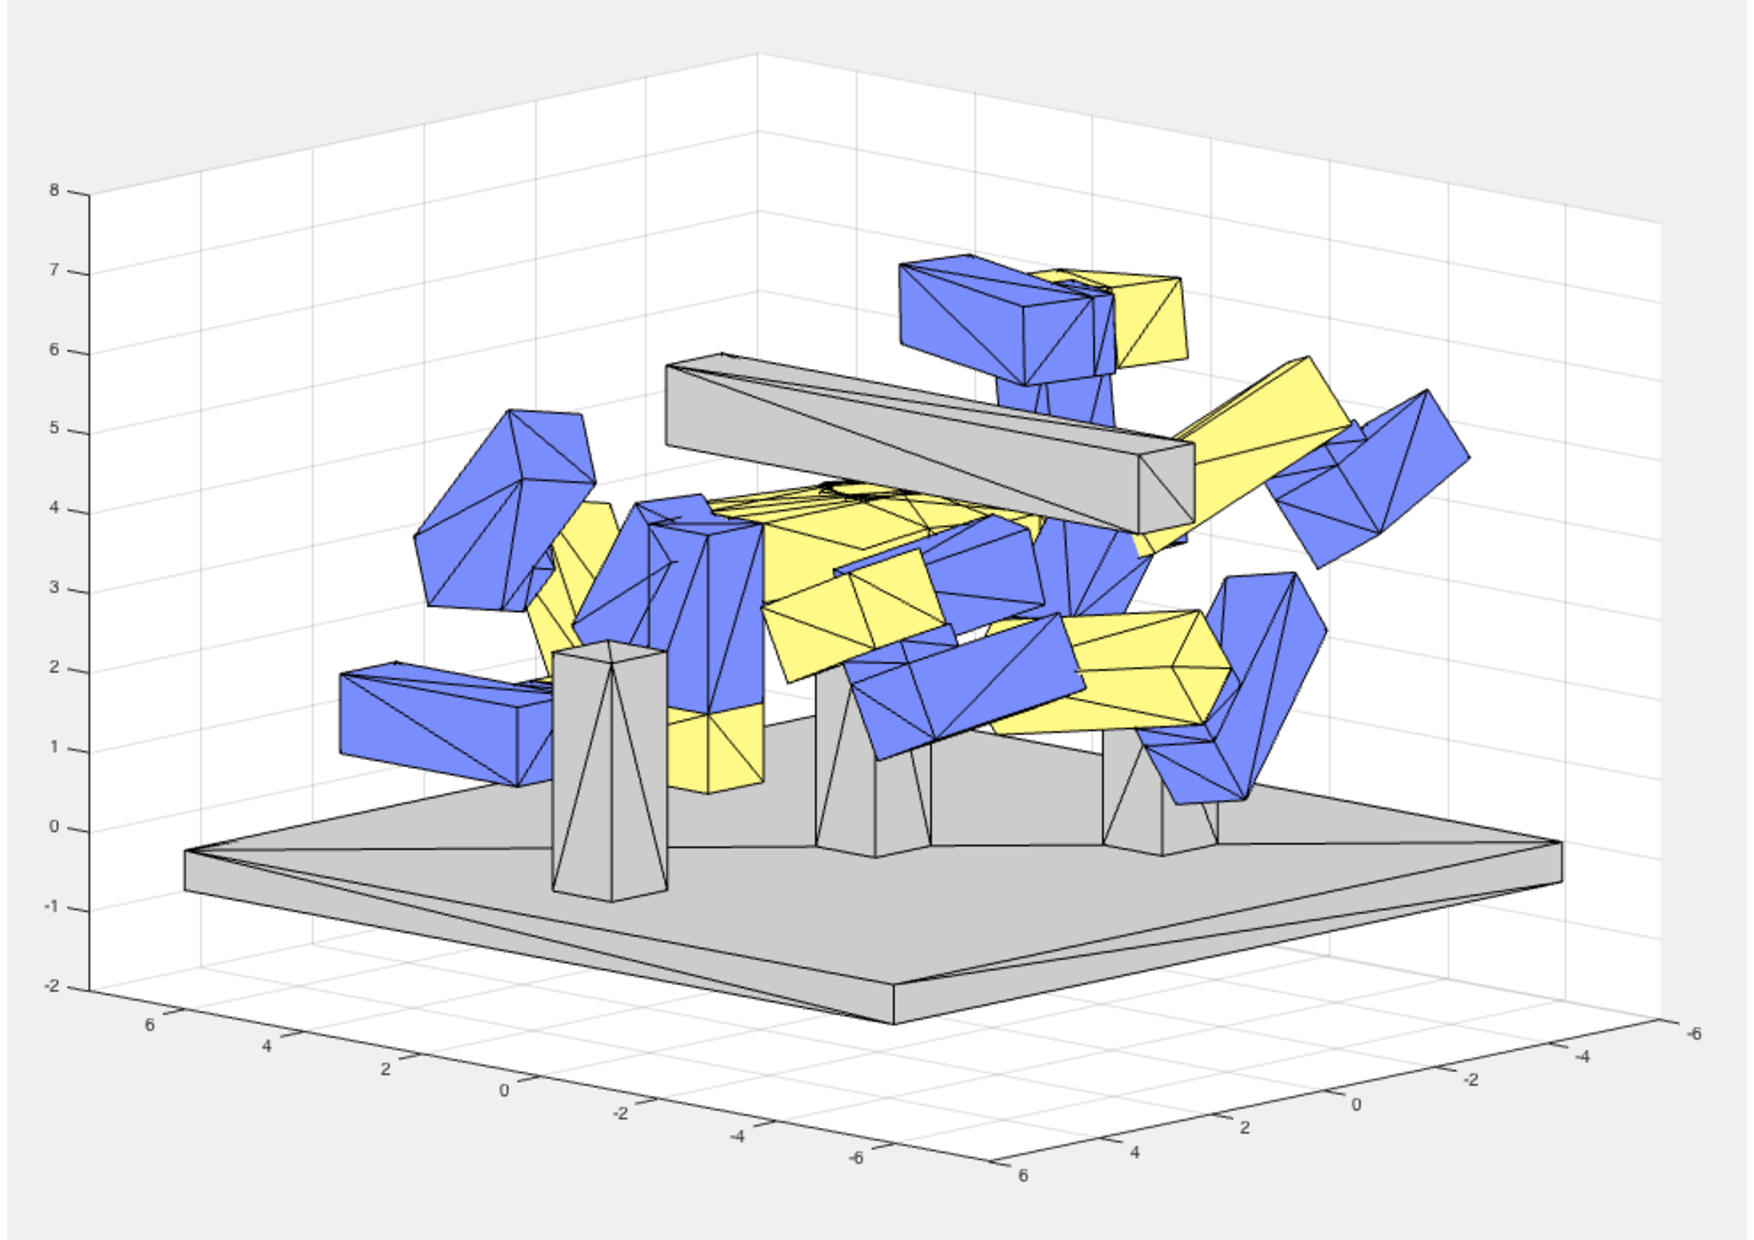
\includegraphics[width=0.5\textwidth]{robotsolution.pdf}
	\caption{PRM generated collision-free movement for a 4-axis robot}
\end{wrapfigure}

Tests have been made for a scenario with a robot with 4 joints. For creating and plotting the environment and the resulting trajectories, Matlab functions are provided.
Because of the dependency on random numbers, the algorithm takes different amounts of time for different runs.
Therefore, 10 runs were made for each version and number of processes.
However, the different versions lead to a different average amount of GPU threads needed.
Hence, to be able to better compare how they scale, the time per number of GPU threads is used as a quantity.
Table 1 shows the results.
One can see, that the version with node communication has a better time to GPU threads ratio, but leads to a greater amount of threads on average.
The versions with less communication, however, have better absolute times.
Furthermore, one sees the improvement from version 2 to version 3 from the asynchronous indicator function.


\begin{table}[h]\label{resulttable}
\centering
\begin{tabular}{| c | c | r | r | r |}

\hline
version	&  processes/	& time (ms)	& GPU 		& time per 1e6  \\ 
		& GPUs		& 			& threads		& GPU threads (ms) \\ 
\hline
		& 1			& 1002		& 696413		& 1448	\\ 
1		& 2			& 763		& 838938		& 918	\\ 
		& 4			& 706		& 1113781	& 647	\\ 
\hline
		& 1			& 900		& 608172		& 1490	\\ 
2		& 2			& 647		& 608172		& 1070	\\ 
		& 4			& 568		& 608172		& 947	\\ 
\hline
		& 1			& 696		& 599847		& 1181	\\ 		
3		& 2			& 554		& 599847		& 951	\\ 
		& 4			& 500		& 599847		& 864	\\ 
\hline

\end{tabular}
\caption{Timing results for the parallelization versions from chapter \ref{solver} on a cluster node with 2x Intel Xeon Six-Core CPU X5650 @2.67GHz and 4x GeForce GTX 480}
\end{table}

As the indicator function has also been implemented on the CPU, all versions could be run without GPU.
In most cases, the GPU code was around 10 times faster. However, the robot code is not optimized for the CPU version, such that this comparison is not quite fair.

\newpage

\bibliographystyle{alpha}
\begin{thebibliography}{999}
	\bibitem{prmlec} D. Burschka, Lecture Robot Motion Planning, source: http://robvis01.informatik.tu-muenchen.de/courses/wegtraj/index.html
	\bibitem{prm1} H. Choset, K. Lynch, S. Hutchinson, G. Kantor, W. Burgard, L. Kavraki and S. Thrun, Principles of Robot Motion: Theory, Algorithms, and Implementation, MIT Press, 2005
	\bibitem{prm2} S. M. LaValle, Planning Algorithms, Cambridge University Press, 2006
	\bibitem{robodyn} T. Buschmann, Skript zur Vorlesung: Roboterdynamik SS14, Lehrstuhl f�r Angewandte Mechanik, TU M�nchen, 2014
	\bibitem{chung} K. Chung, Wenping Wang, Quick Collision Detection of Polytopes in Virtual Environments, Proceedings of the ACM Symposium on Virtual Reality Software and Technology (VRST 96), Mark Green (ed.), 1996
	\bibitem{ericson} C. Ericson, Real-Time Collision Detection, Elsevier, 2005
\end{thebibliography}

\end{document}


















